\iffalse
\let\negmedspace\undefined
\let\negthickspace\undefined
\documentclass[journal,12pt,twocolumn]{IEEEtran}
\usepackage{cite}
\usepackage{amsmath,amssymb,amsfonts,amsthm}
\usepackage{algorithmic}
\usepackage{graphicx}
\usepackage{textcomp}
\usepackage{xcolor}
\usepackage{txfonts}
\usepackage{listings}
\usepackage{enumitem}
\usepackage{mathtools}
\usepackage{gensymb}
\usepackage{comment}
\usepackage[breaklinks=true]{hyperref}
\usepackage{tkz-euclide}
\usepackage{listings}
\usepackage{gvv}
\def\inputGnumericTable{}
\usepackage[latin1]{inputenc}
\usepackage{color}
\usepackage{array}
\usepackage{longtable}
\usepackage{calc}
\usepackage{multirow}
\usepackage{hhline}
\usepackage{ifthen}
\usepackage{lscape}
\usepackage{circuitikz}

\newtheorem{theorem}{Theorem}[section]
\newtheorem{problem}{Problem}
\newtheorem{proposition}{Proposition}[section]
\newtheorem{lemma}{Lemma}[section]
\newtheorem{corollary}[theorem]{Corollary}
\newtheorem{example}{Example}[section]
\newtheorem{definition}[problem]{Definition}
\newcommand{\BEQA}{\begin{eqnarray}}
\newcommand{\EEQA}{\end{eqnarray}}
\newcommand{\define}{\stackrel{\triangle}{=}}
\theoremstyle{remark}
\newtheorem{rem}{Remark}
\begin{document}

\bibliographystyle{IEEEtran}
\vspace{3cm}

\title{Gate 2022- Instrumentation Engineering}
\author{EE23BTECH11058 - Sindam Ananya$^{*}$% <-this % stops a space
}
\maketitle
\newpage
\bigskip

\renewcommand{\thefigure}{\theenumi}
\renewcommand{\thetable}{\theenumi}

\vspace{3cm}
\textbf{Question 11:} 
The input $x(t)$ to a system is related to its output $y(t)$ as \\ \\
$\dfrac{dy(t)}{dt} + y(t) = 3x(t-3)u(t-3)$\\ \\
Here $u(t)$ represents a unit-step function.\\
The transfer function of this system is 
\begin{enumerate}
\item[(A)] $\frac{e^{-3s}}{s+3}$\\
\item[(B)] $\frac{3e^{-3s}}{s+1}$\\
\item[(C)] $\frac{3e^{-\brak{s/3}}}{s+1}$\\
\item[(D)] $\frac{e^{-\brak{s/3}}}{s+3}$
\end{enumerate}
\hfill{(GATE IN 2022)}\\
\solution
\fi
\begin{align}
\frac{dy(t)}{dt} + y(t) = 3x(t-3)u(t-3)
\end{align}
By applying Laplace Transform on both sides\\
\begin{align}
x(t) &\xleftrightarrow{\mathcal{L}} X(s)\\
x(t-t_o) &\xleftrightarrow{\mathcal{L}} X(s)e^{-st_o}\\
sY(s) + Y(s) &= 3X(s)e^{-3s}\\
Y(s)\brak{s+1} &= 3X(s)e^{-3s}\\
H(s) = \frac{Y(s)}{X(s)} &= \frac{3e^{-3s}}{s+1} \quad \brak{Re(s)>0}\\
H(j\omega) &= \frac{3e^{-3j\omega}}{1+j\omega}\\
&= \frac{3\brak{cos3\omega - jsin3\omega}}{1+j\omega}\\
\lvert{H(j\omega)} \rvert&= \frac{3}{\sqrt{1+\omega^{2}}}\\
phase &= \tan^{-1}\brak{\frac{\omega \cos(3\omega) + \sin(3\omega)}{\omega \sin(3\omega) - \cos(3\omega)}}
\end{align}
\begin{figure}[h!]
    \centering
    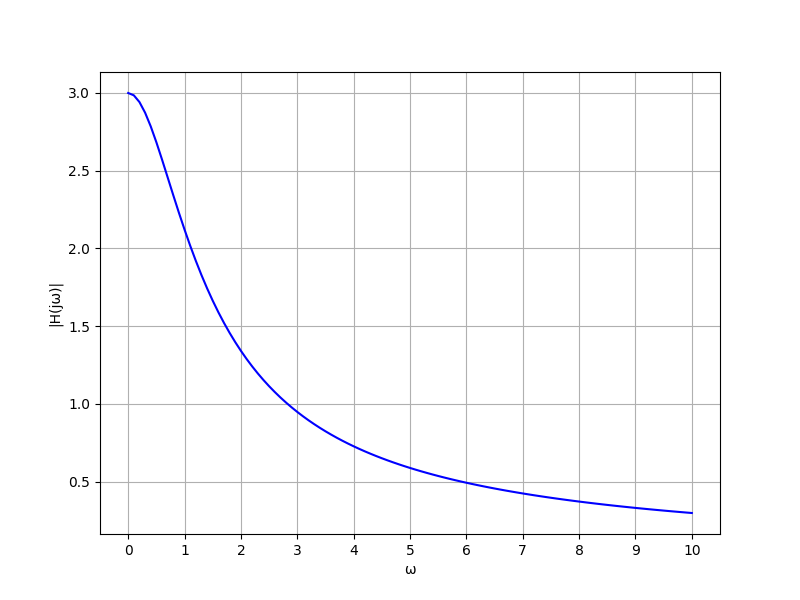
\includegraphics[width=\columnwidth]{2022/IN/11/figs/freq.png}
    \caption{Plot for magnitude of transfer function}
    \label{fig:gate2022in11fig1}
\end{figure}
\begin{figure}[h!]
    \centering
    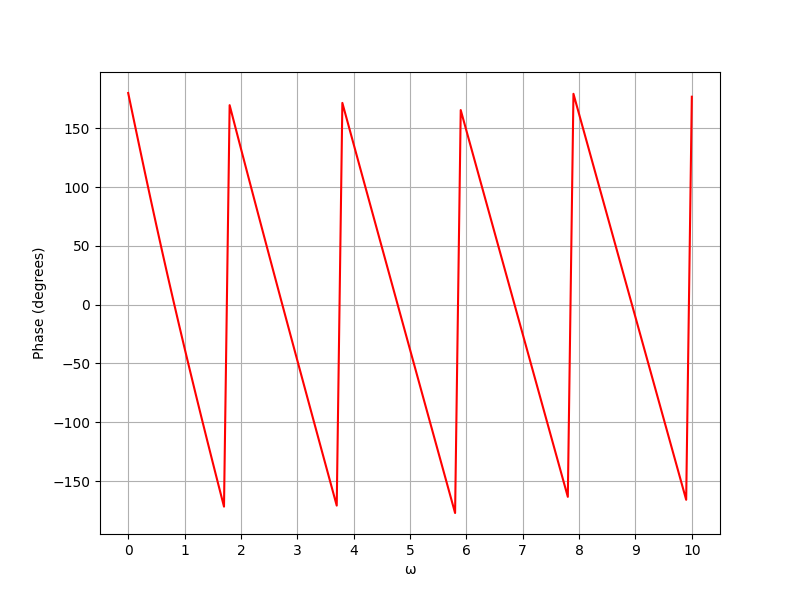
\includegraphics[width=\columnwidth]{2022/IN/11/figs/phase.png}
    \caption{Plot for phase of transfer function}
    \label{fig:gate2022in11fig2}
\end{figure}
%\end{document}
